\section{平:北海道カーテン}

\subsection{歴史}
事件が起こったのは2018年8月20日である。オガワインティライミの友人が沖縄を訪れた際、オガワインティライミが国際通りにある「平カーテン」という店の写真を撮ってきてくれと頼んだことから事態は急展開した。その写真は図\ref{tairakaten}である。


\begin{figure}[H]
  \centering
  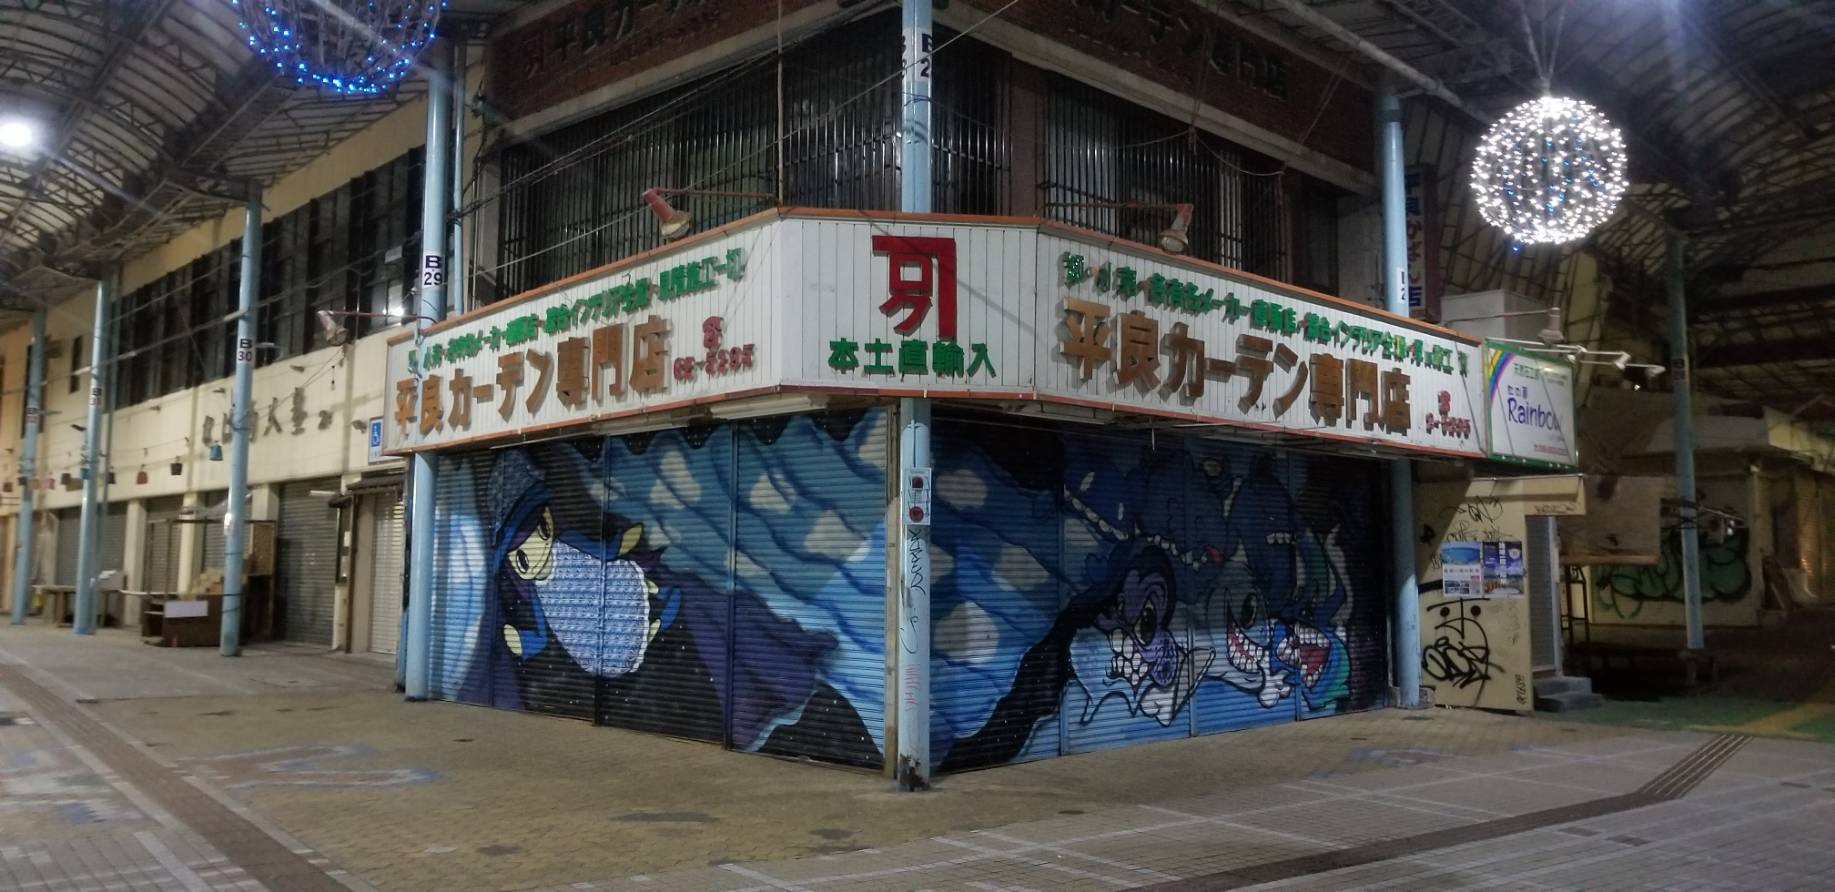
\includegraphics[clip,scale=0.2]{./section/Taira/figures/tairakaten.jpg}
  \caption{平カーテン}
\label{tairakaten}
\end{figure}

オガワインティライミ氏は、この写真を又吉氏、武田学長に披露したことにより、その後の裁判に発展するような大問題となる疑惑が大浮上したのである。以下に、その疑惑が浮上した瞬間を示す。\par

2018/08/20(月)\par
\par
2:11	希望新風	\[写真\] \par
2:11	希望新風	\[写真\] \par
5:26	又吉康平	買い物しなさい\par
10:49	Kosuke Takeda	あ、ここ北海道でみたことあるぞ、、、?\par
12:25	又吉康平	[写真]\par
12:25	又吉康平	なはと書いてある\par
13:10	Kosuke Takeda	「なは」と書いているだけで、北海道支店なのだろう。\par
16:55	希望新風	現在、ポが優勢{\sf (´\_ゝ`)}\par
\par
2018/08/21(火)\par
\par
24:45	希望新風	北海道、で確定でよろしいでしょうか{\sf (´\_ゝ`)}笑\par
5:37	又吉康平	https://tairacurtain.ti-da.net 沖縄だぞ\par
13:43	Kosuke Takeda	なるほど、なるほど、、、\par
なんと、似た店が沖縄にもあるとは\par
13:43	Kosuke Takeda	[写真]\par
13:51	又吉康平	[写真]\par
13:59	Kosuke Takeda	看板には「62-5295」と書いてあり、頭に "8" を足すということは正確な結果に繋がらないのではないでしょうか。そこには「沖縄」という思い込み・バイアスが入り込む余地があると考えます。\par
つまり、電話番号を検索対象とする場合は、正確に何の先入観(バイアス)もなく探索するために、「62-5295」とのみ打ち込む必要があると考えます。\par
2018/08/22(水)\par
\par
4:57	希望新風	マタヨ選手、敗北か…?{\sf (´\_ゝ`)}笑\par
6:03	又吉康平	62-5295で出て来るのも別の会社か店じゃん\par
2018/08/24(金)\par
\par
13:01	希望新風	沖縄に決定か…?{\sf (´\_ゝ`)}笑\par

こうして、又吉被告の出身地は沖縄なのか、北海道なのか、はたまた別の地なのかを問う裁判が行われることとなった。


\subsection{議事録}

\begin{figure}[H]
  \centering
  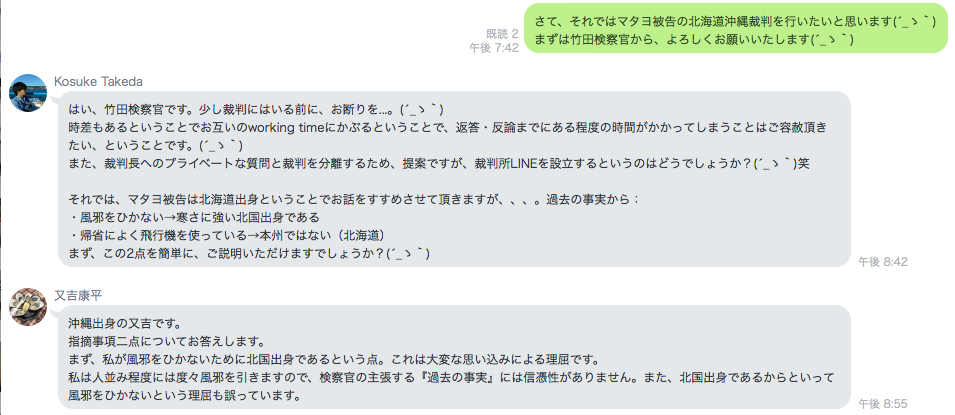
\includegraphics[clip,scale=0.5]{./section/Taira/figures/giji1.png}
  \caption{議事録1}
\label{giji1}
\end{figure}

\begin{figure}[H]
  \centering
  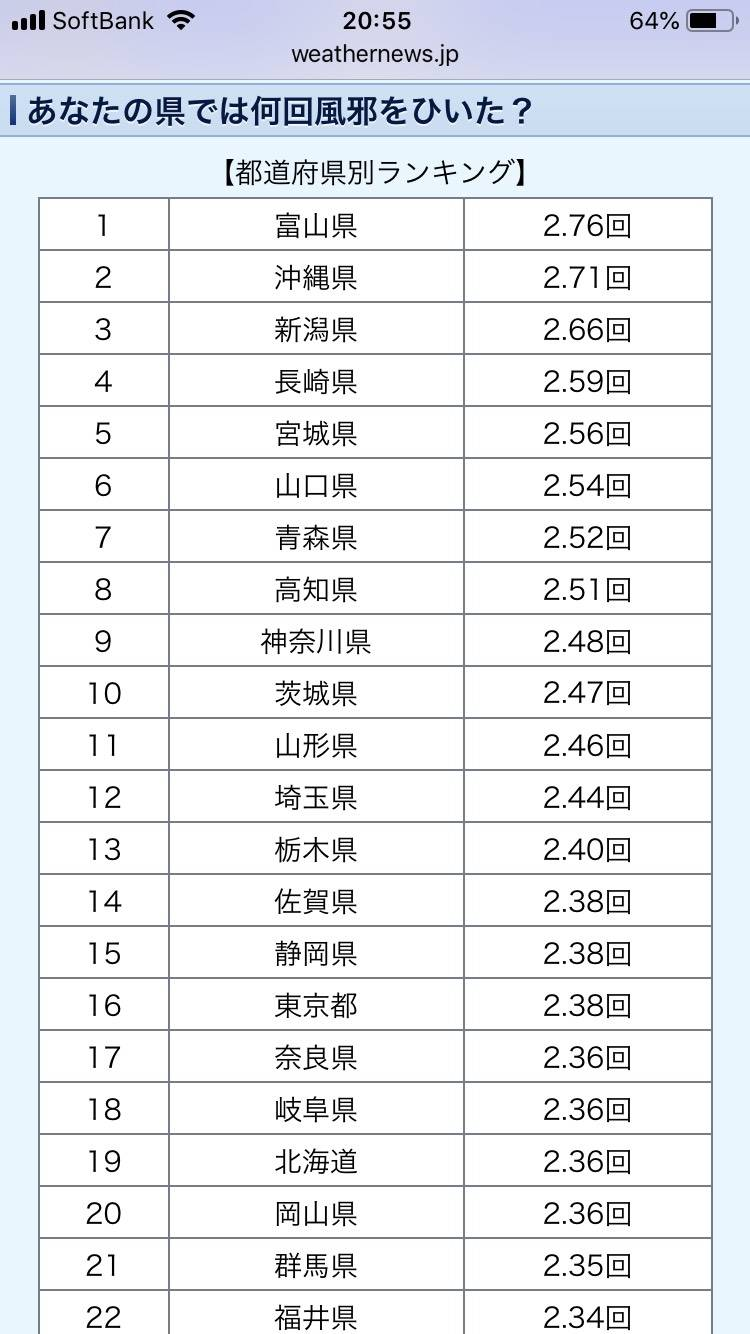
\includegraphics[clip,scale=0.2]{./section/Taira/figures/fig1}
  \caption{証拠1}
\label{fig1}
\end{figure}

\begin{figure}[H]
  \centering
  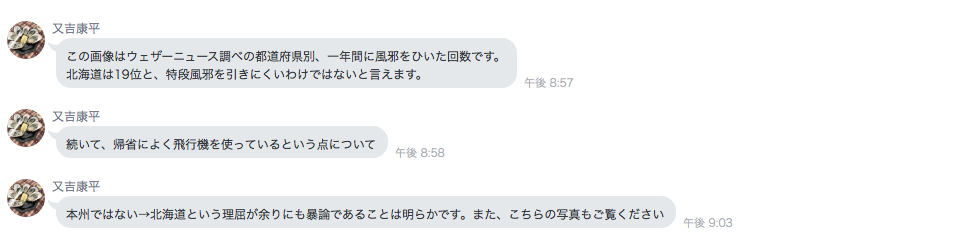
\includegraphics[clip,scale=0.5]{./section/Taira/figures/giji2.png}
  \caption{議事録2}
\label{giji2}
\end{figure}

\begin{figure}[H]
  \centering
  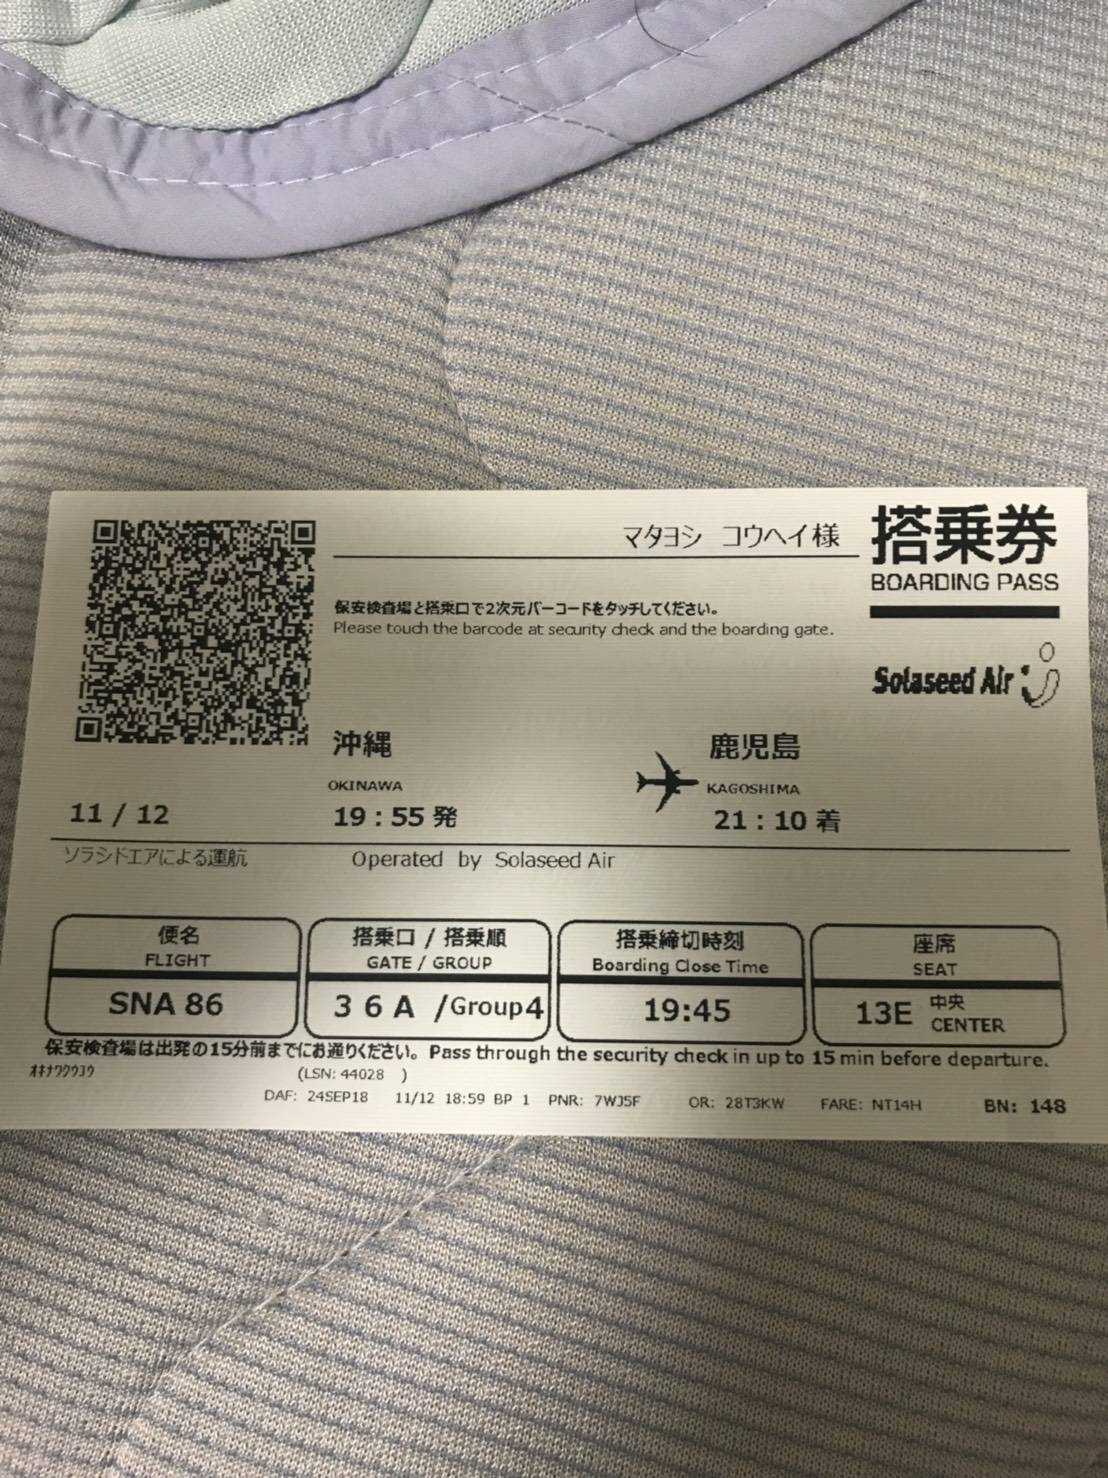
\includegraphics[clip,scale=0.2]{./section/Taira/figures/fig2}
  \caption{証拠2}
\label{fig2}
\end{figure}

\begin{figure}[H]
  \centering
  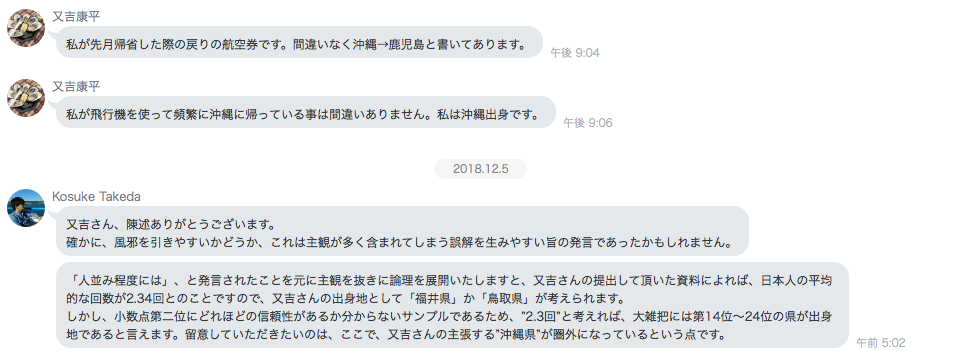
\includegraphics[clip,scale=0.5]{./section/Taira/figures/giji3.png}
  \caption{議事録3}
\label{giji3}
\end{figure}

\begin{figure}[H]
  \centering
  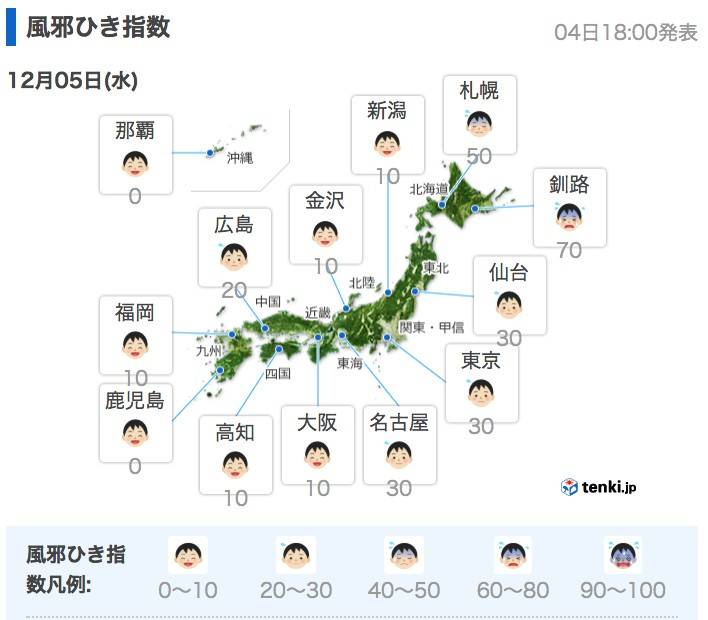
\includegraphics[clip,scale=0.2]{./section/Taira/figures/fig3}
  \caption{証拠3}
\label{fig3}
\end{figure}

%\newpage
\begin{figure}[H]
  \centering
  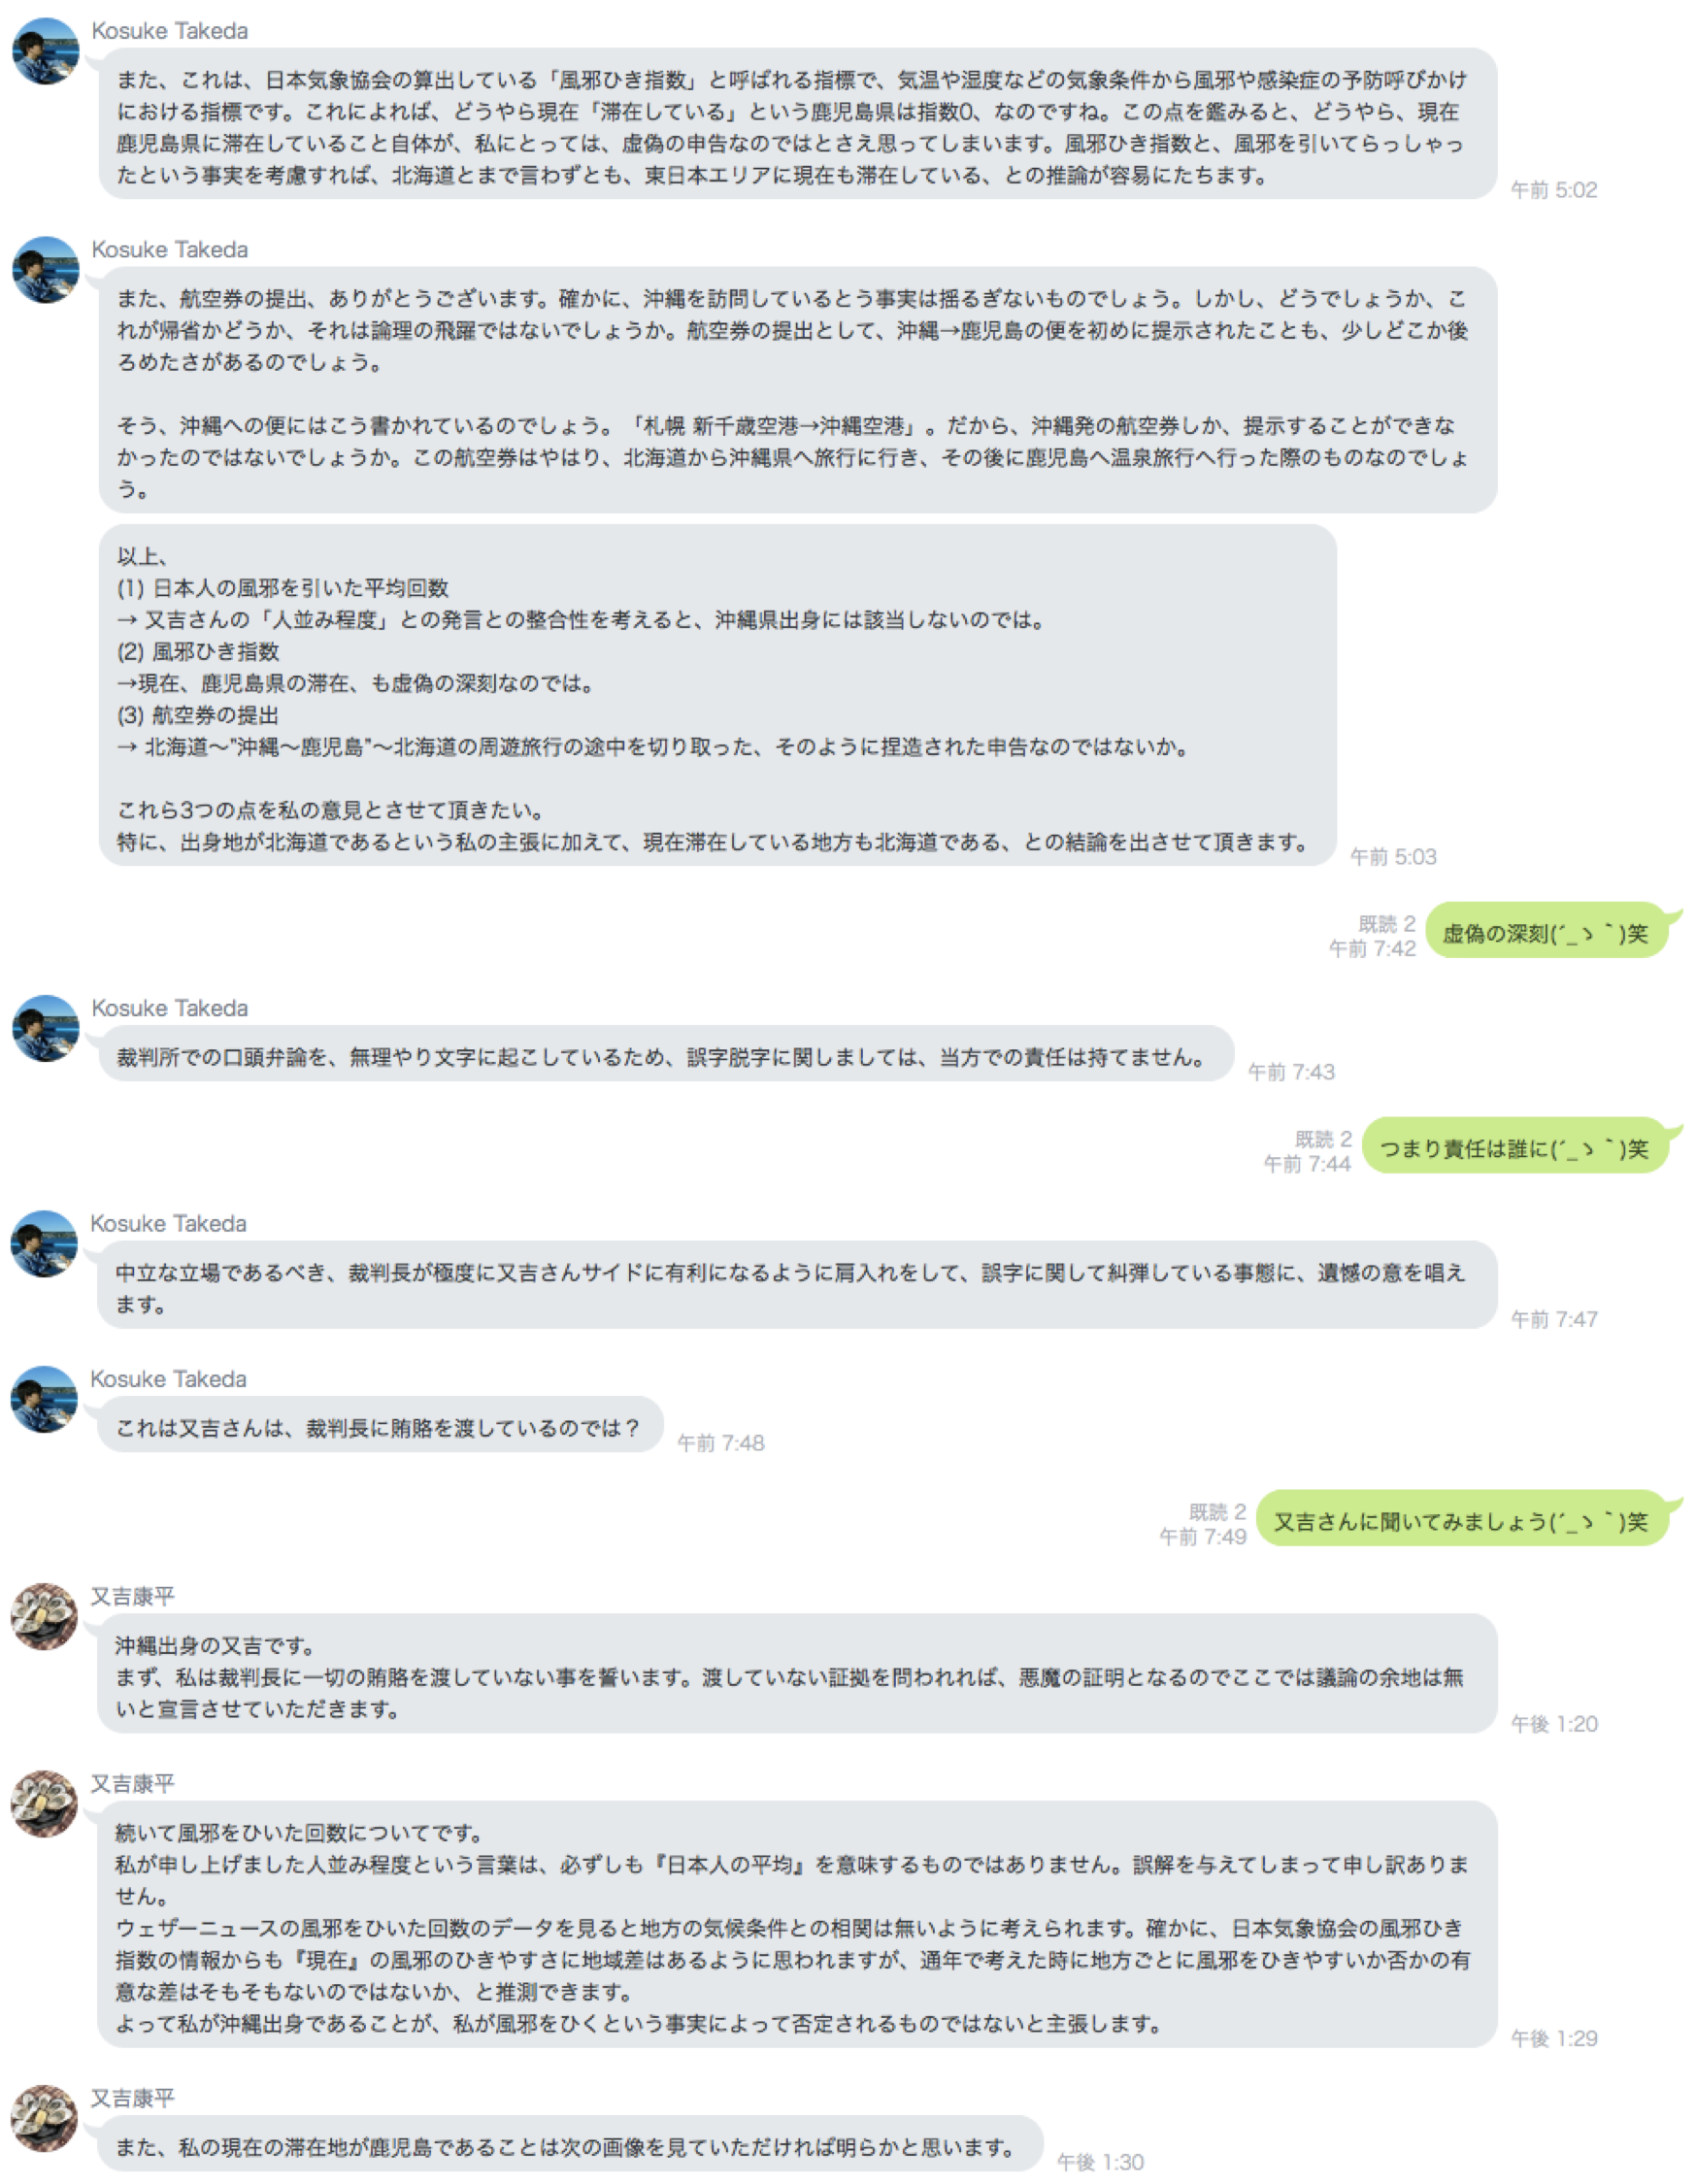
\includegraphics[clip,scale=0.5]{./section/Taira/figures/giji4.png}
  \caption{議事録4}
\label{giji4}
\end{figure}

\begin{figure}[H]
  \centering
  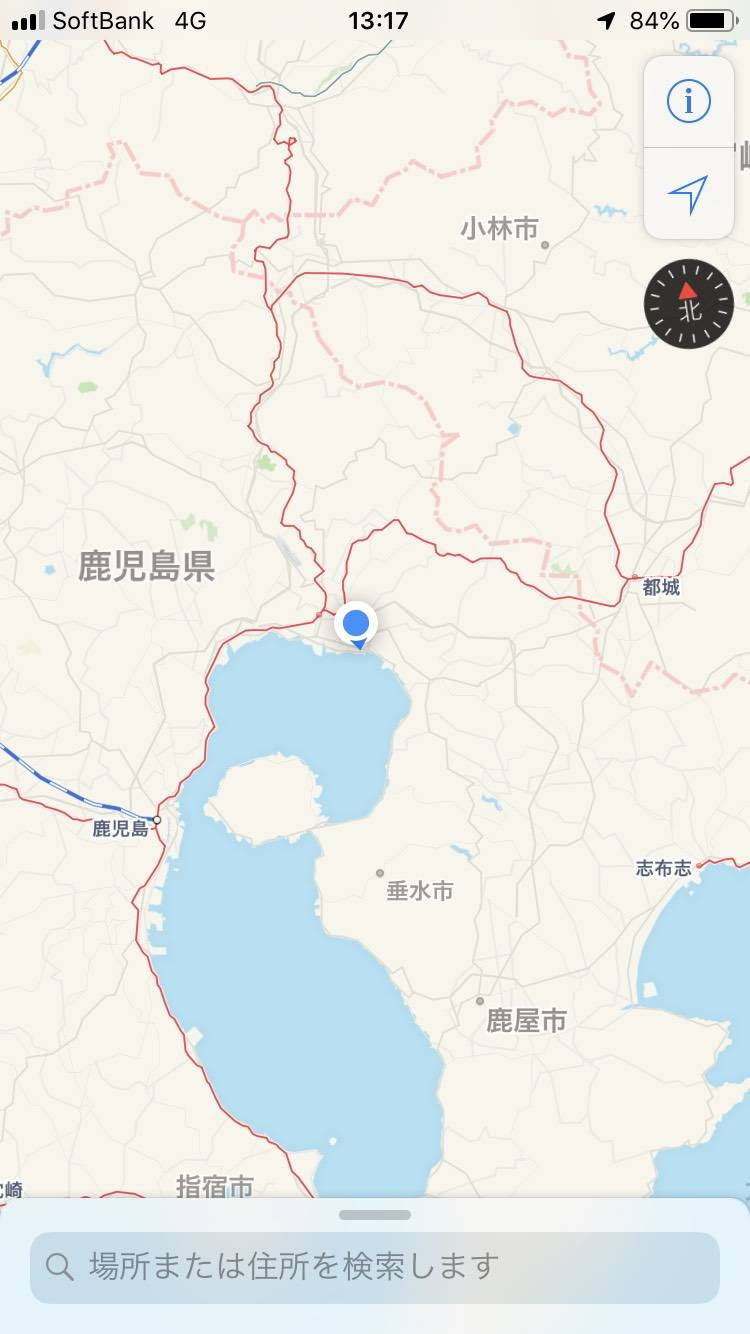
\includegraphics[clip,scale=0.2]{./section/Taira/figures/fig4}
  \caption{証拠4}
\label{fig4}
\end{figure}

\begin{figure}[H]
  \centering
  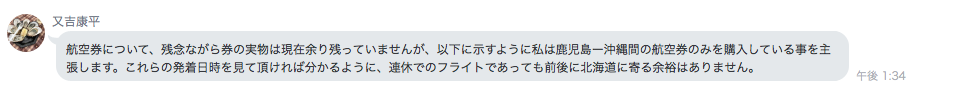
\includegraphics[clip,scale=0.5]{./section/Taira/figures/giji5}
  \caption{議事録5}
\label{giji5}
\end{figure}

\begin{figure}[H]
  \centering
  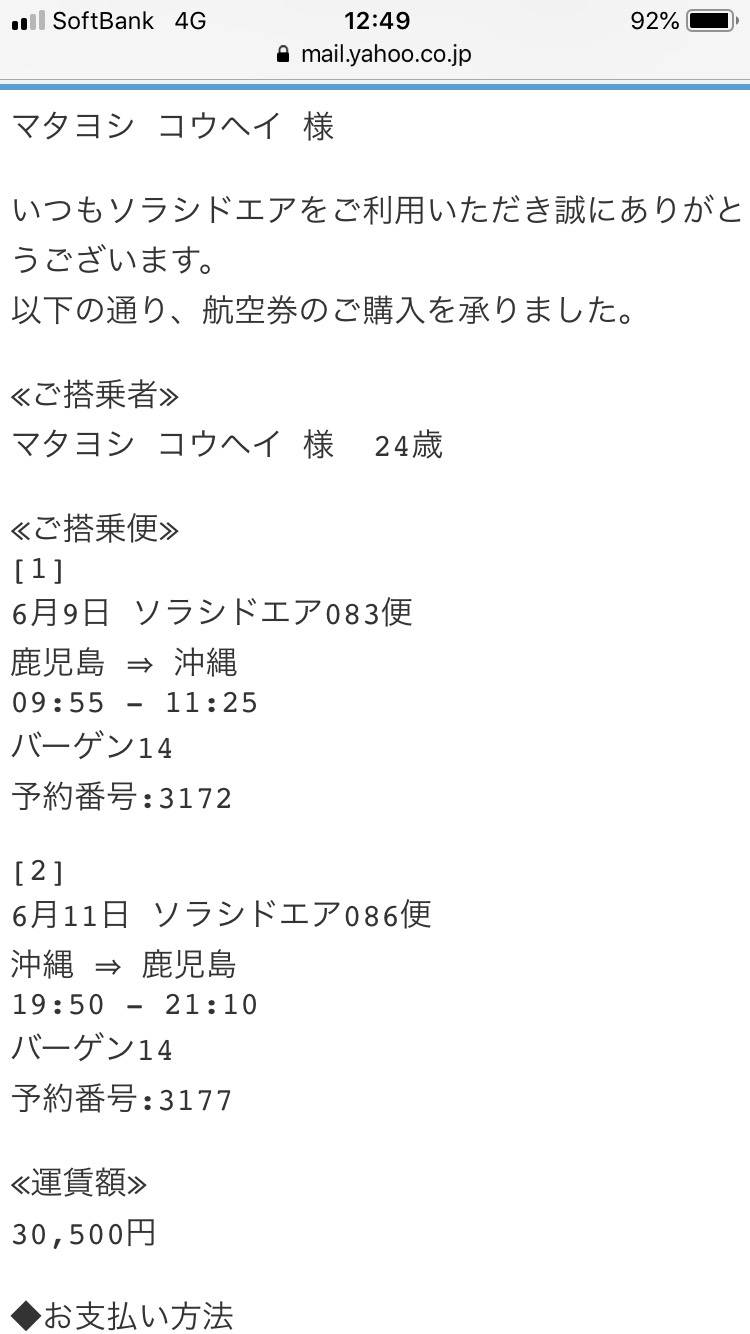
\includegraphics[clip,scale=0.2]{./section/Taira/figures/fig5}
  \caption{証拠5}
\label{fig5}
\end{figure}

\begin{figure}[H]
  \centering
  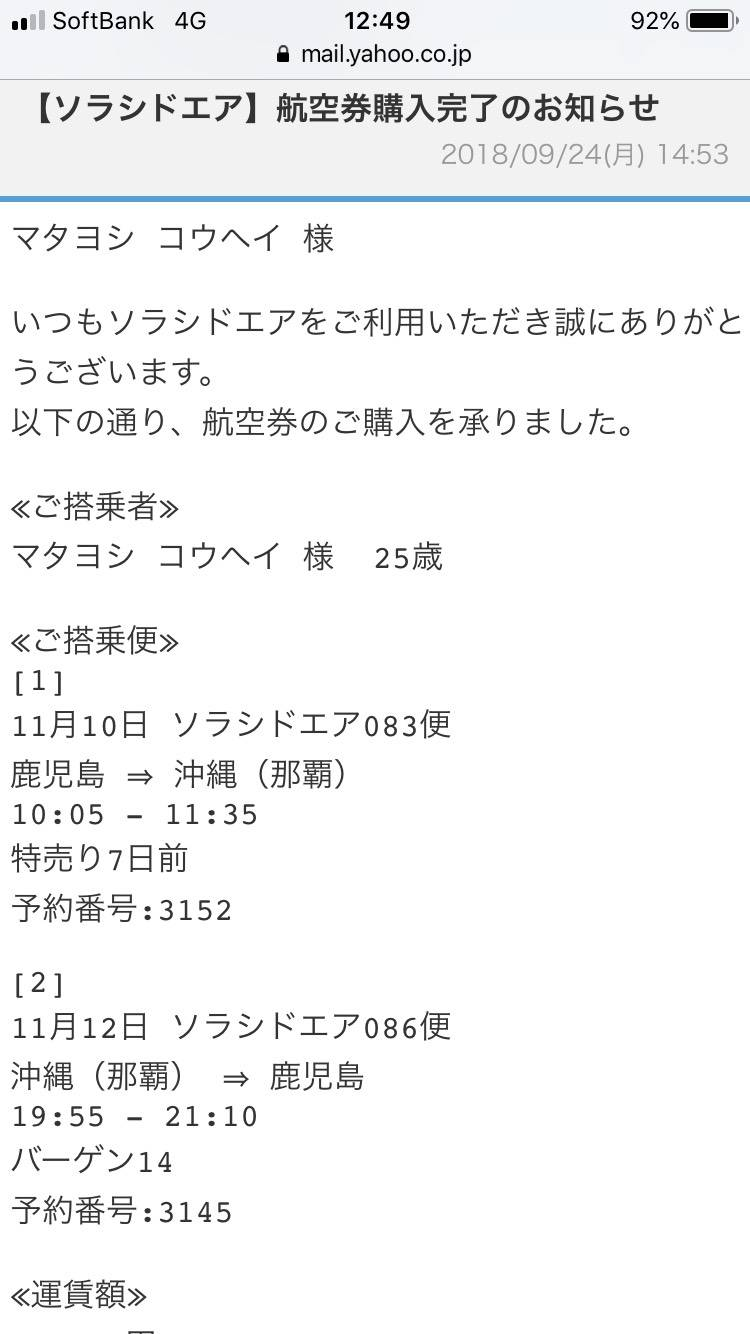
\includegraphics[clip,scale=0.2]{./section/Taira/figures/fig6}
  \caption{証拠6}
\label{fig6}
\end{figure}

\begin{figure}[H]
  \centering
  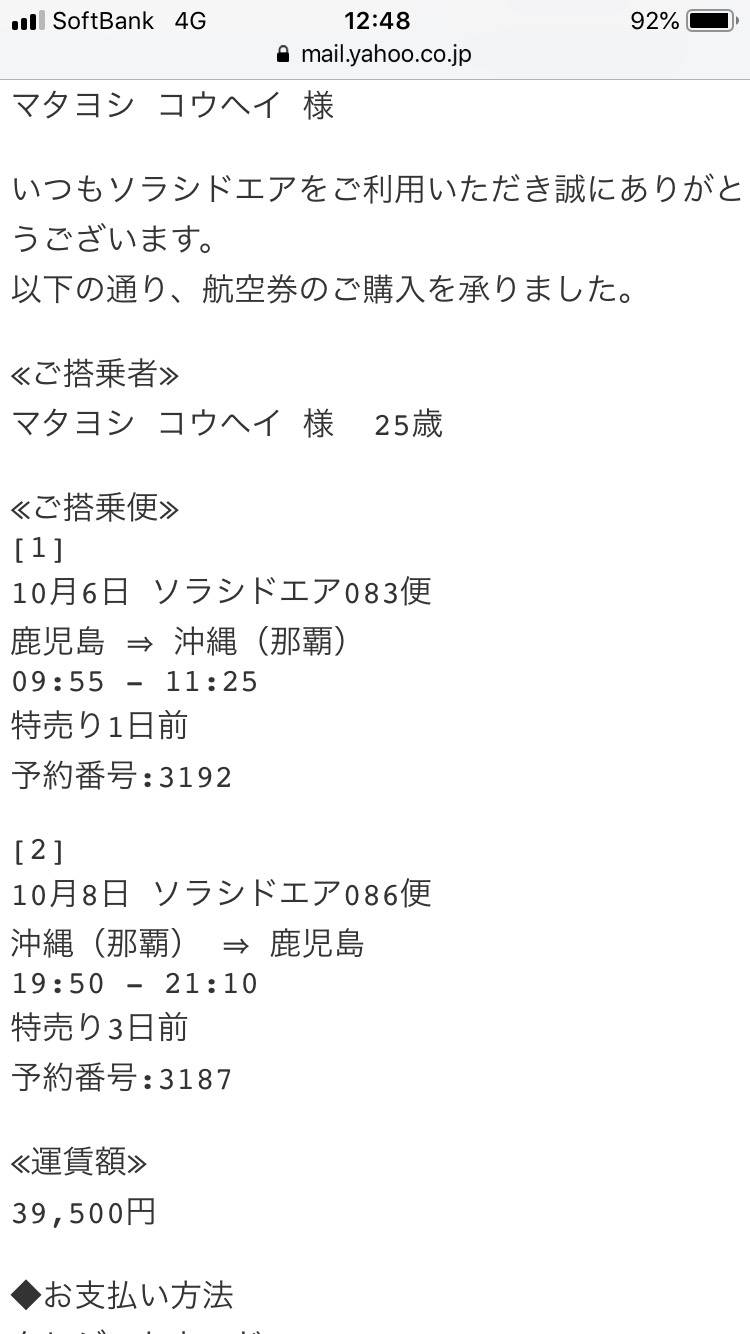
\includegraphics[clip,scale=0.2]{./section/Taira/figures/fig7}
  \caption{証拠7}
\label{fig7}
\end{figure}

\begin{figure}[H]
  \centering
  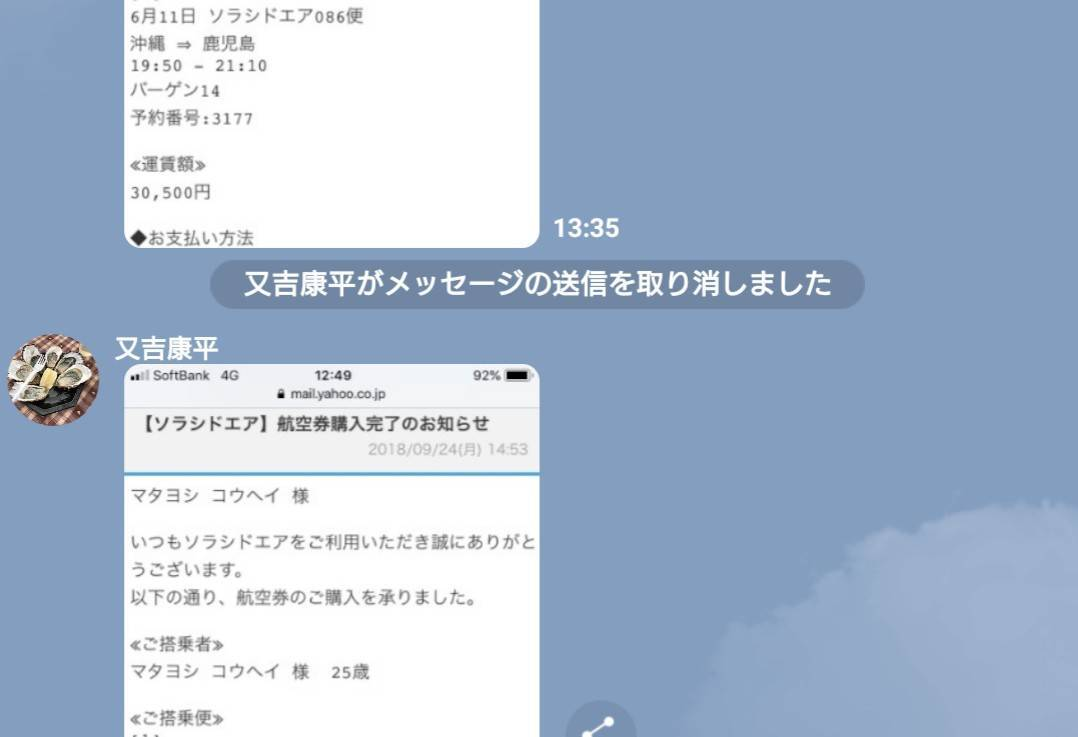
\includegraphics[clip,scale=0.2]{./section/Taira/figures/fig8}
  \caption{証拠8}
\label{fig8}
\end{figure}

\begin{figure}[H]
  \centering
  
\includegraphics[clip,scale=0.5]{./section/Taira/figures/giji9}
  \caption{議事録9}
\label{giji9}
\end{figure}

\begin{figure}[H]
  \centering
  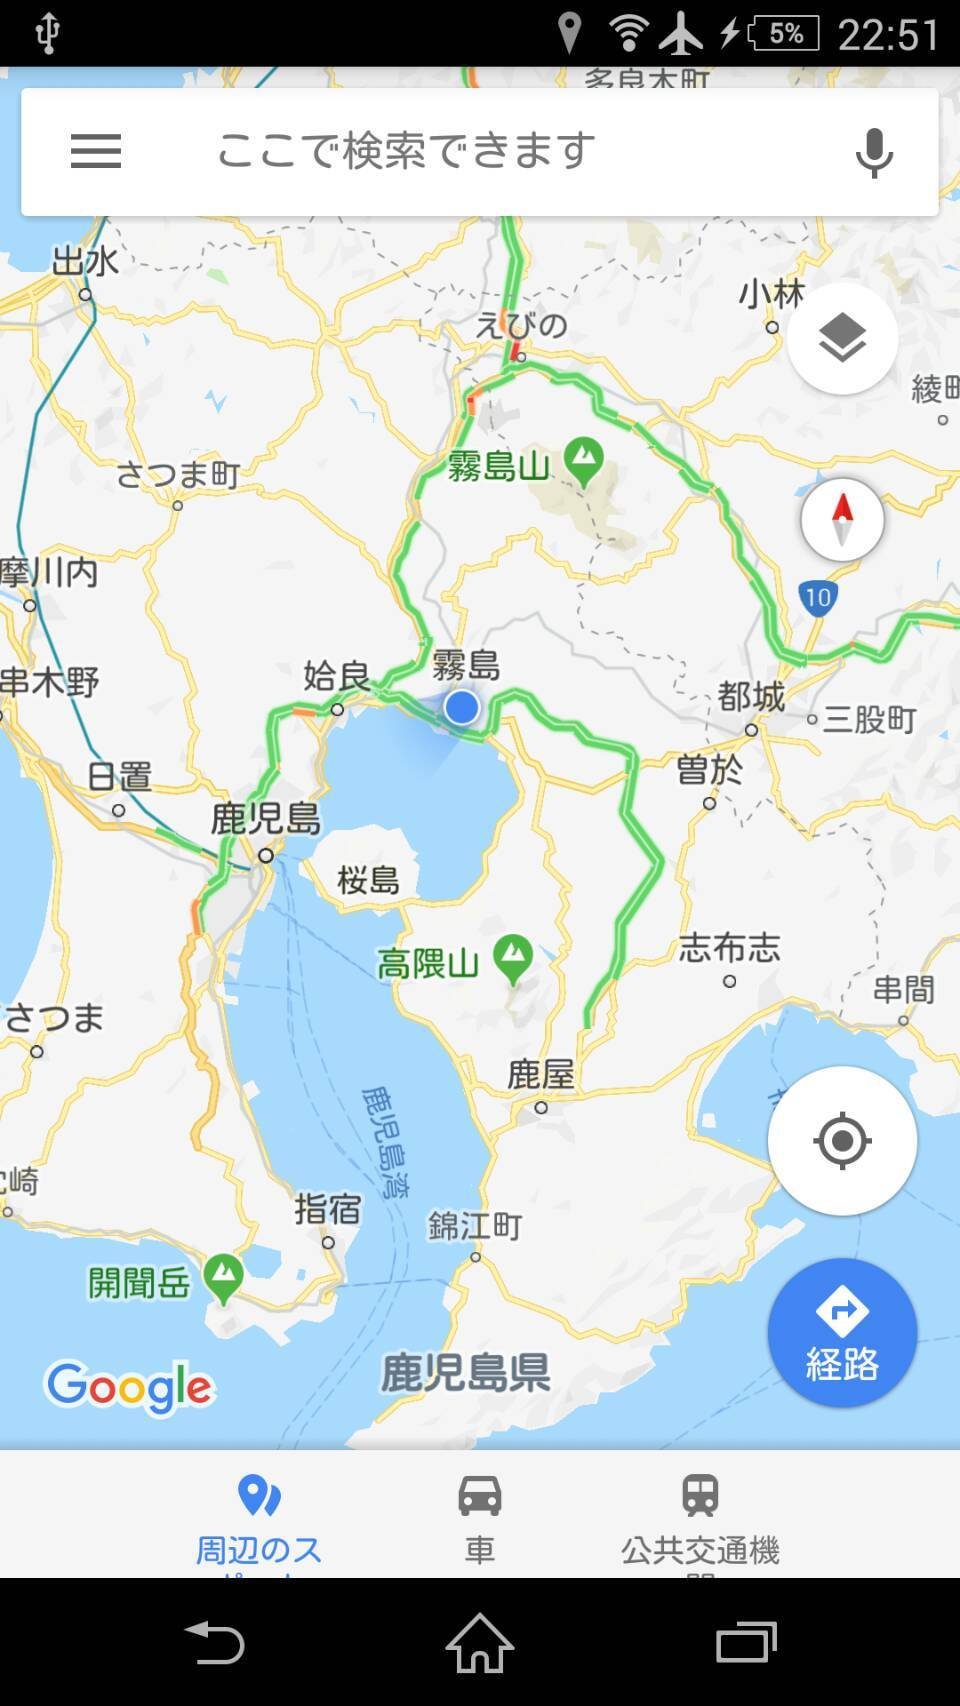
\includegraphics[clip,scale=0.2]{./section/Taira/figures/fig9}
  \caption{証拠9}
\label{fig9}
\end{figure}


\begin{figure}[H]
  \centering
  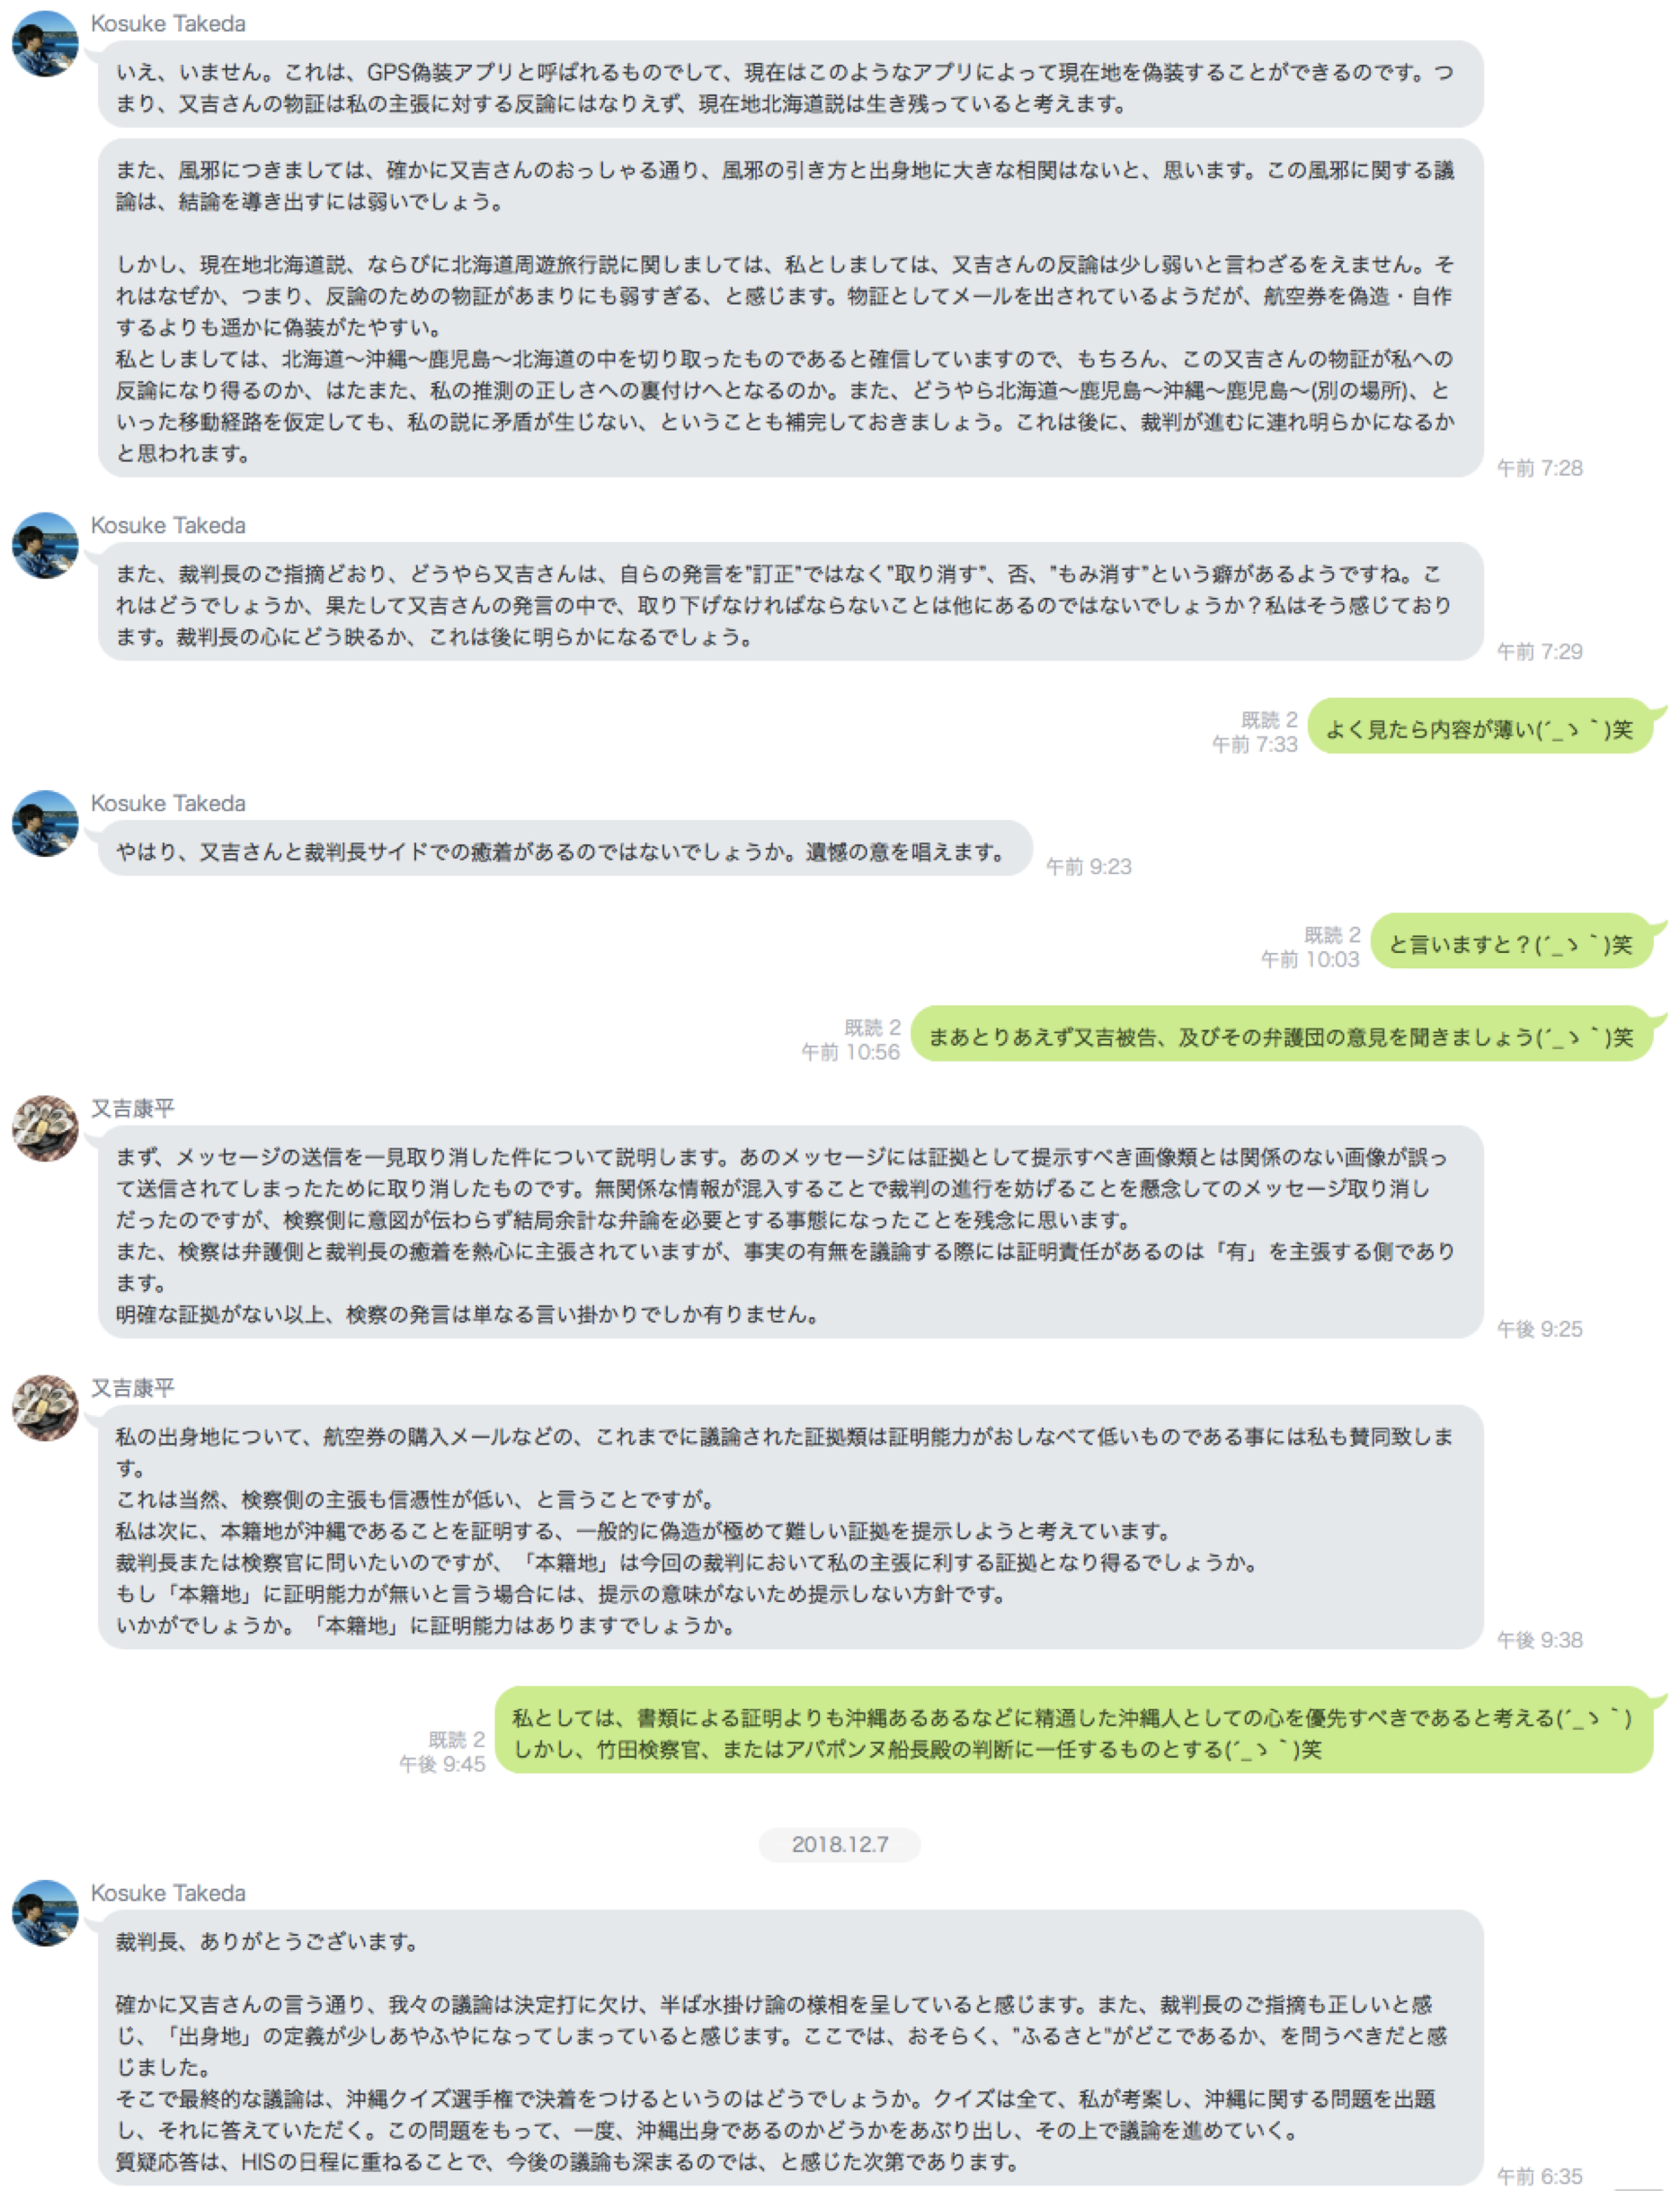
\includegraphics[clip,scale=0.5]{./section/Taira/figures/giji101}
  \caption{議事録10}
\label{giji101}
\end{figure}

\begin{figure}[H]
  \centering
  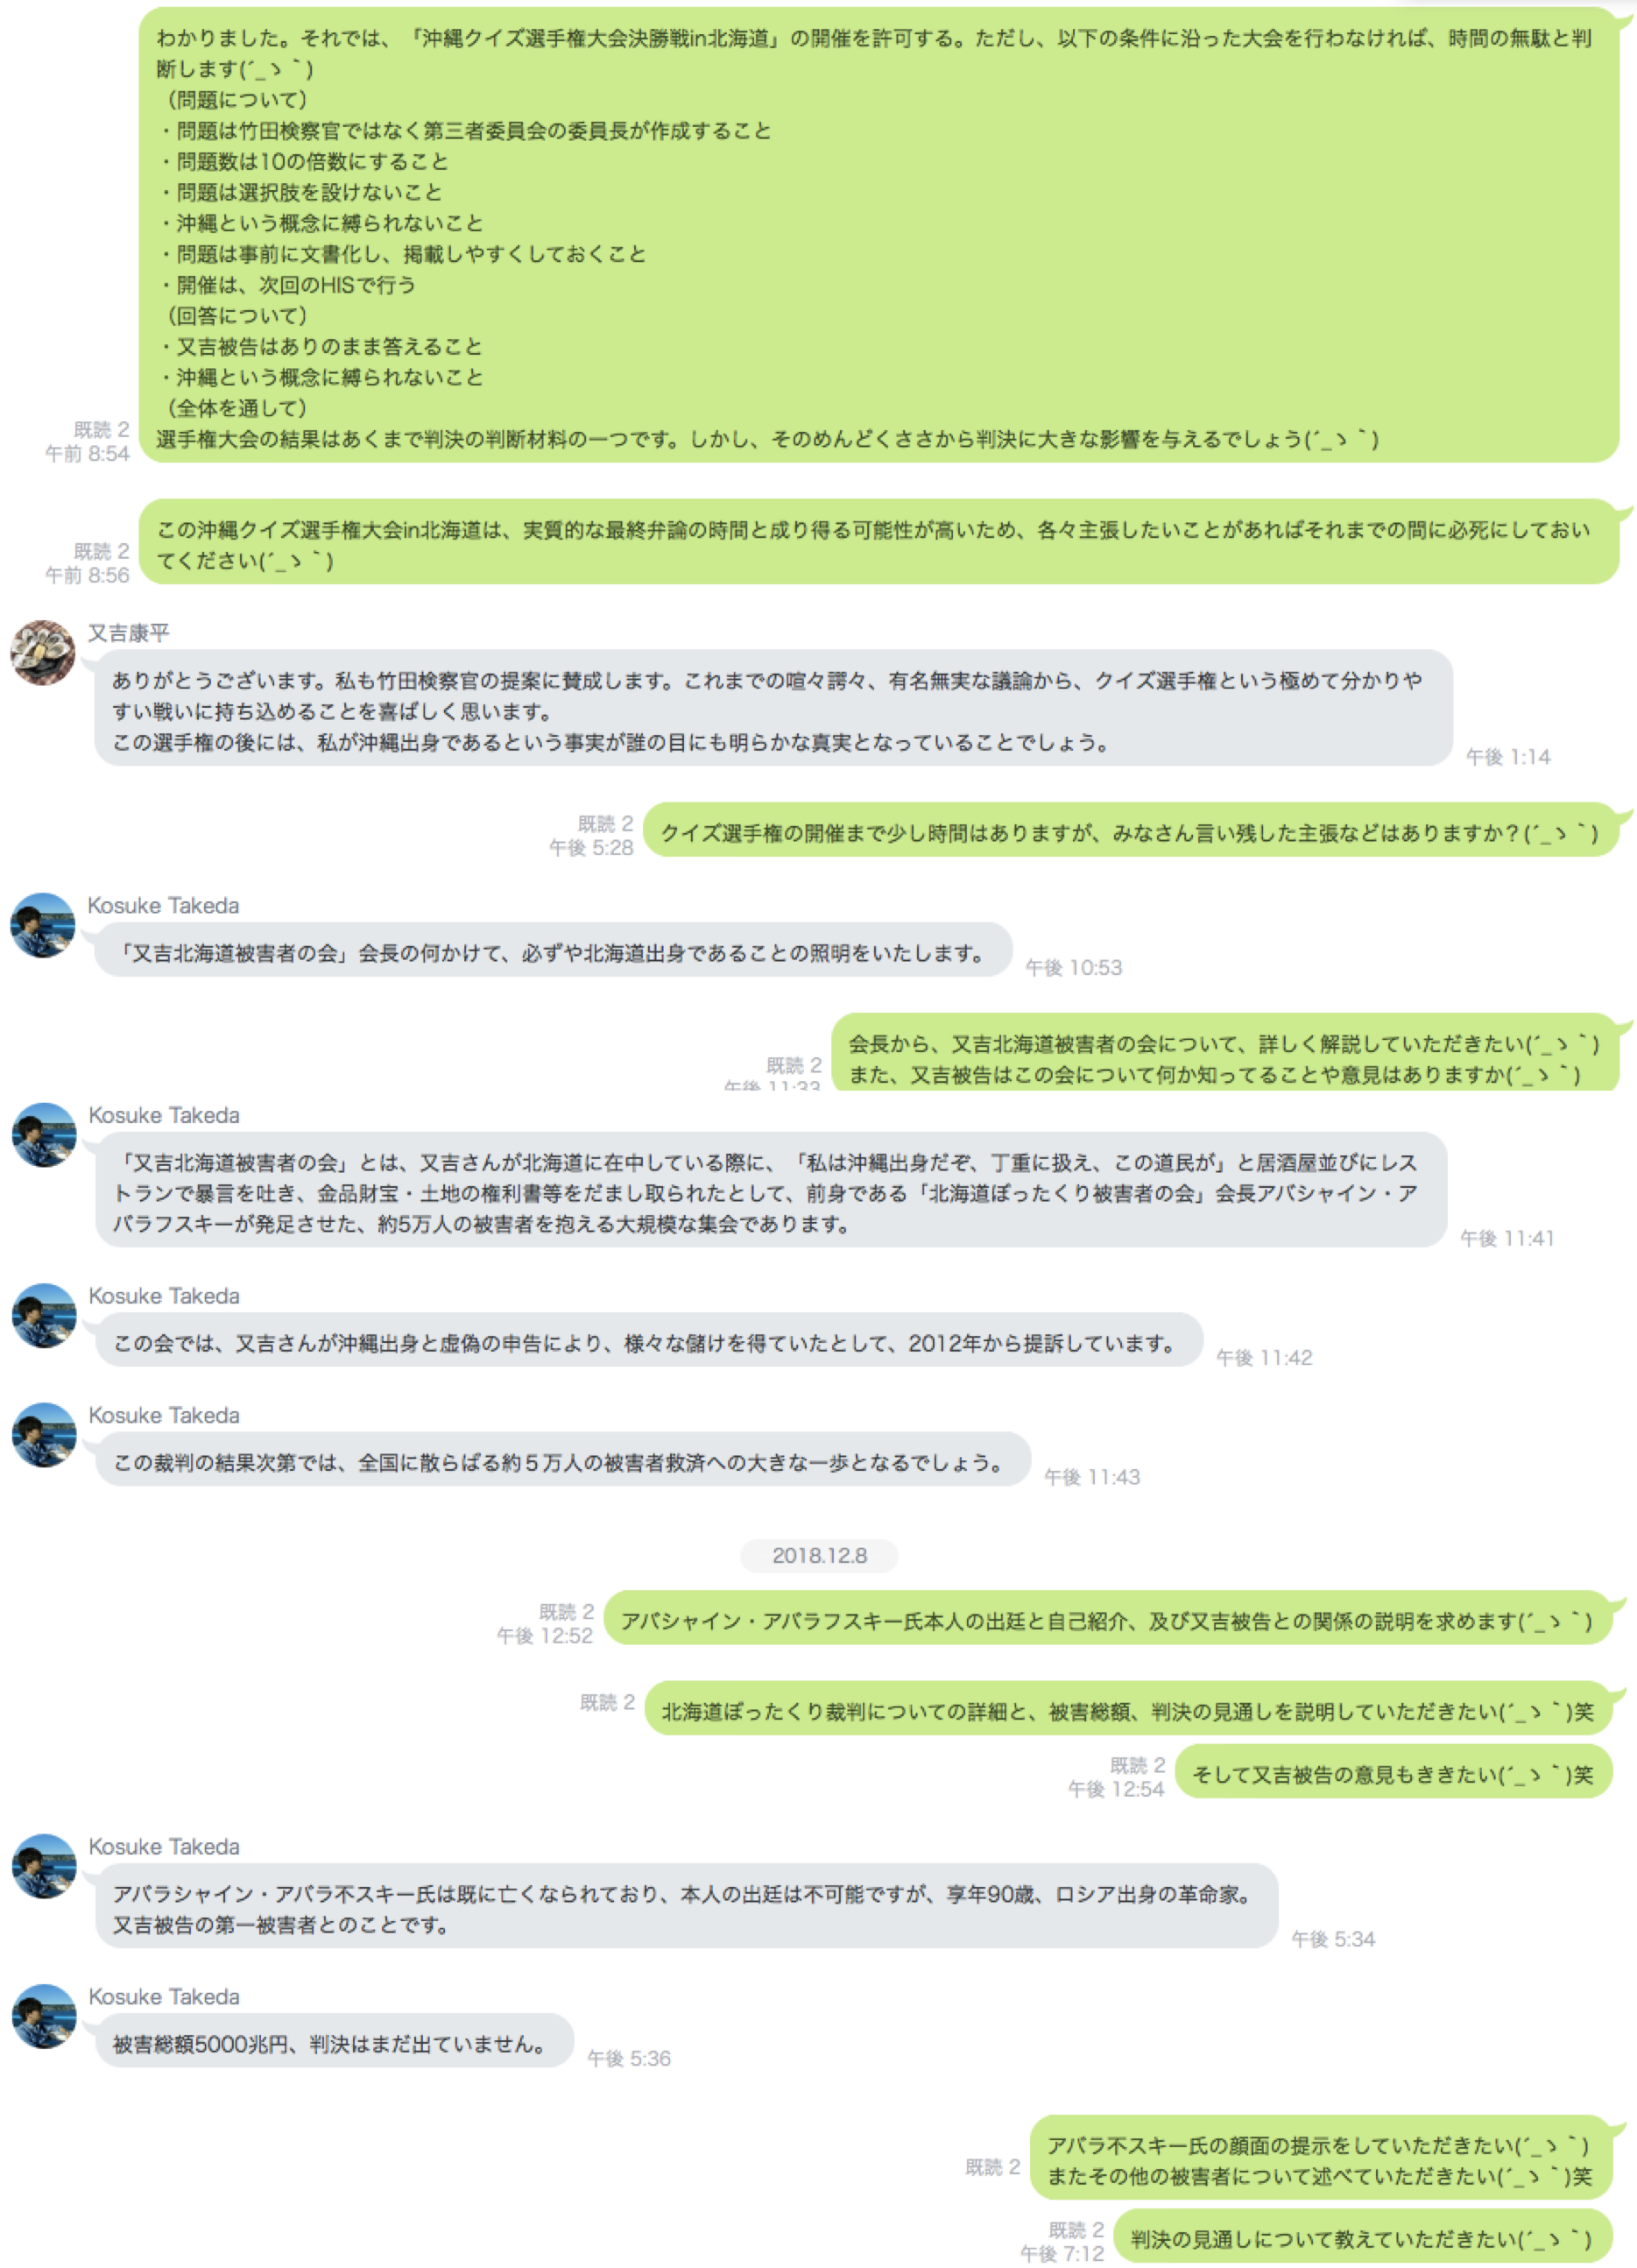
\includegraphics[clip,scale=0.5]{./section/Taira/figures/giji102}
  \caption{議事録11}
\label{giji102}
\end{figure}

\begin{figure}[H]
  \centering
  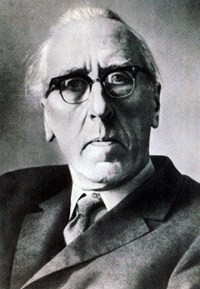
\includegraphics[clip,scale=0.7]{./section/Taira/figures/fig10}
  \caption{証拠10}
\label{fig10}
\end{figure}


\begin{figure}[H]
  \centering
  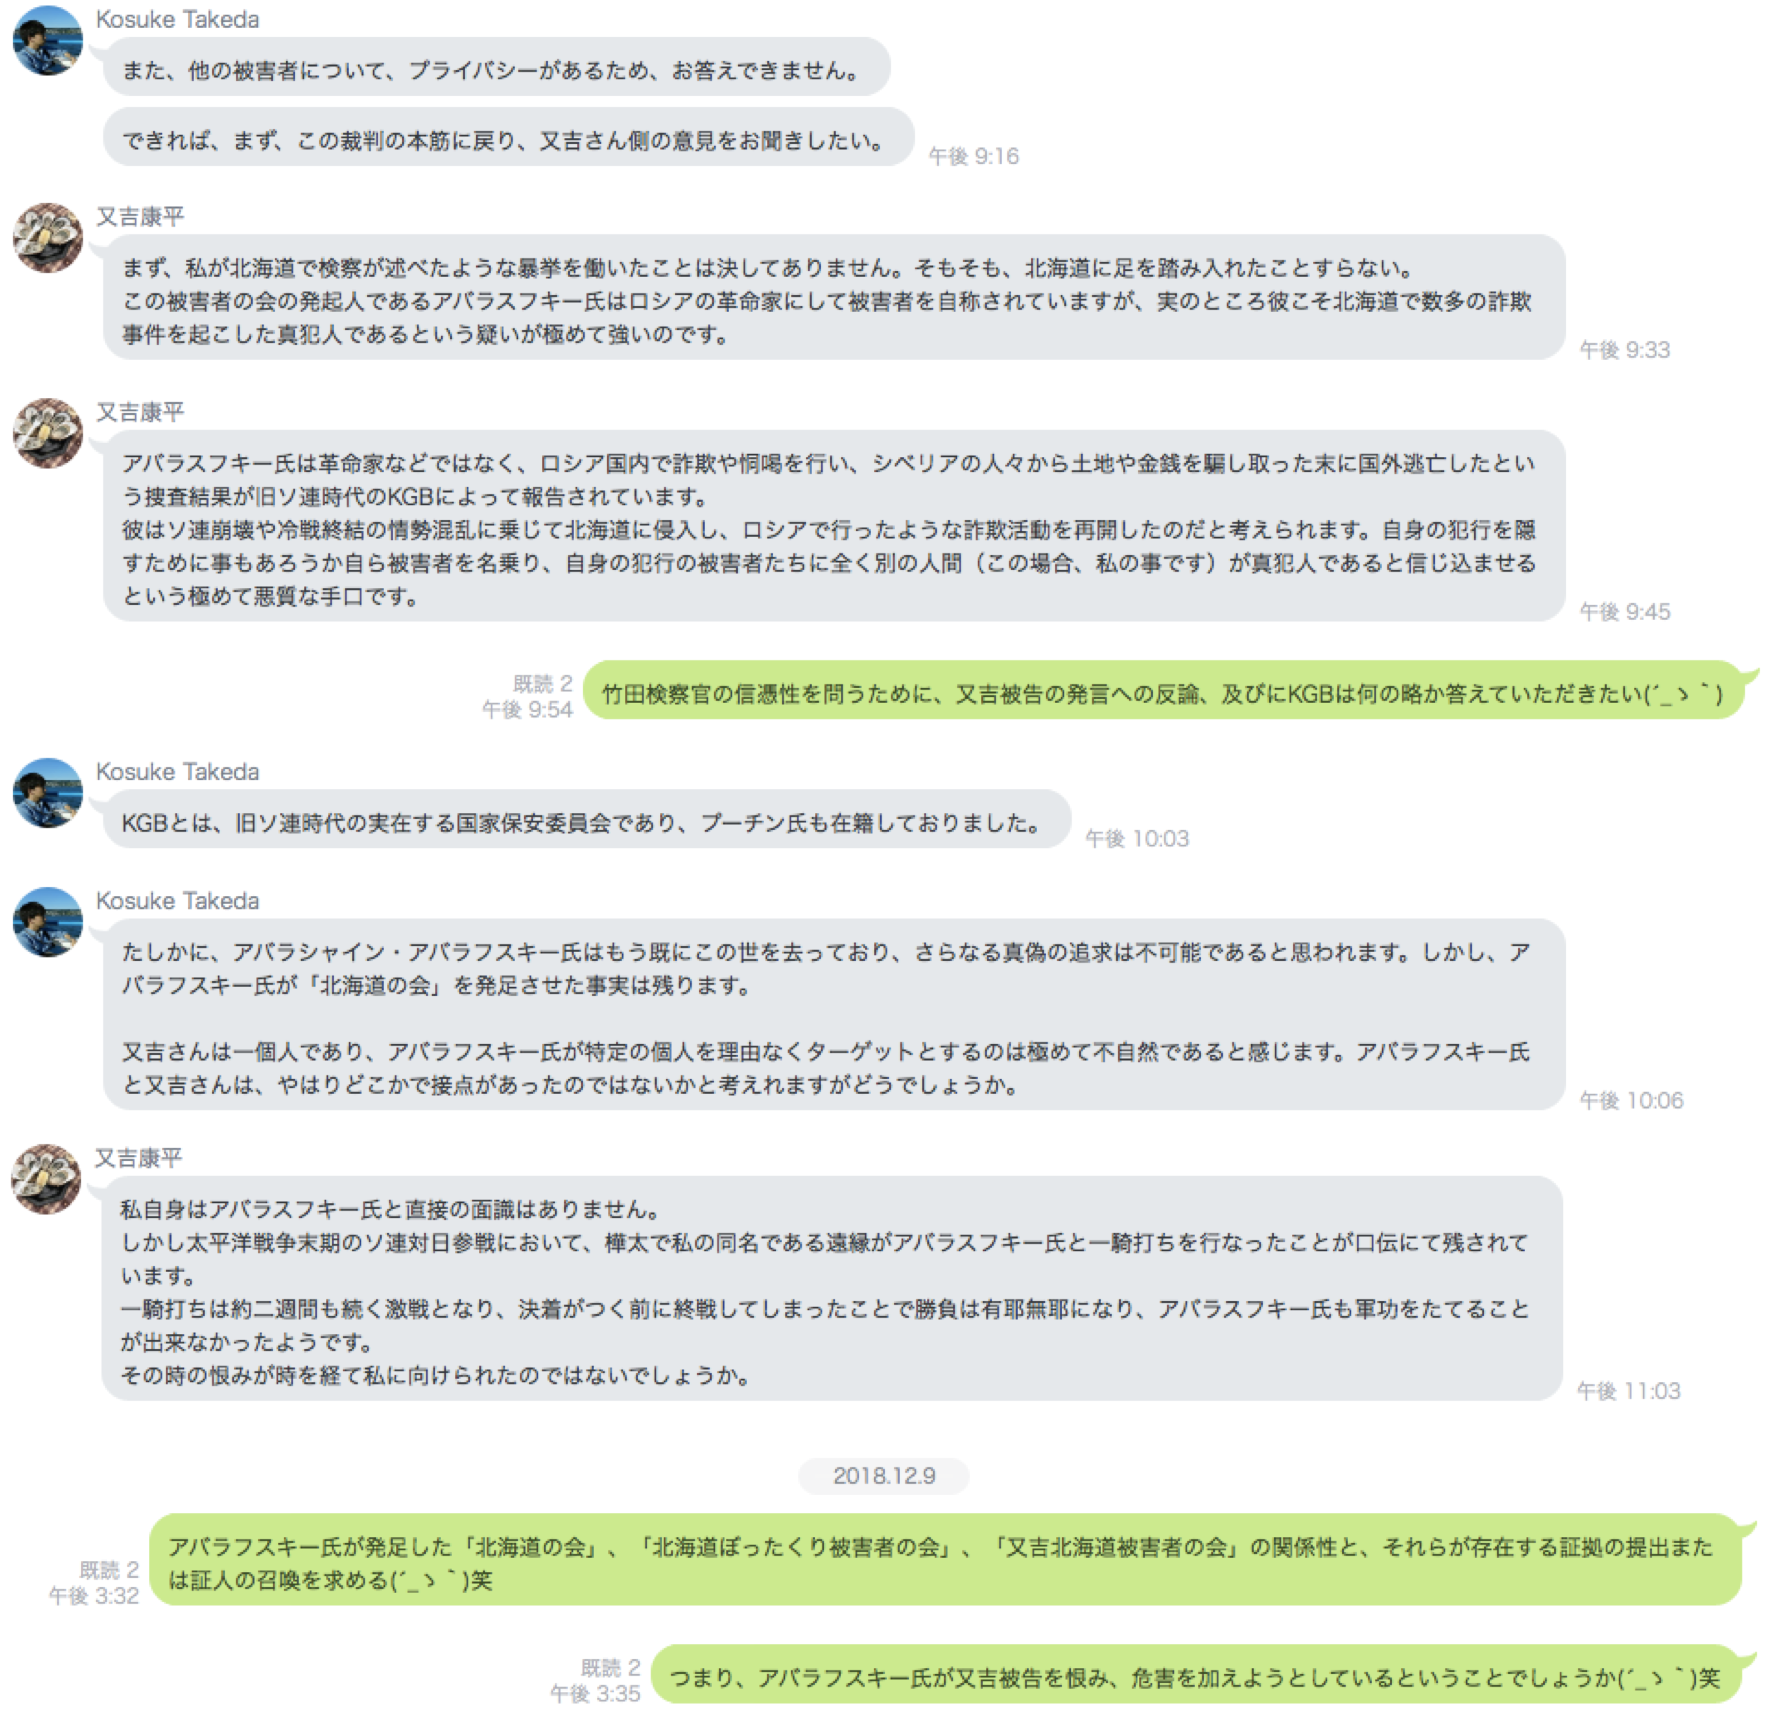
\includegraphics[clip,scale=0.5]{./section/Taira/figures/giji11}
  \caption{議事録12}
\label{giji11}
\end{figure}

(裁判長)又吉北海道裁判を始めたいと思います。又吉被告、何か主張はありますか\par
(又吉被告)私は沖縄出身です。生まれたのは沖縄県那覇市前島。前島。もともと干潟みたいなとこで、埋め立てたところ。\par
(裁判長)じゃあ、武田検事、何かありますか。\par
(武田検事)又吉被告は虚偽の申告で、訴えることにしました。又吉被告は数々の虚偽の申告により、大学時代に友人たちを騙していました。そこで沖縄・北海道に関する質疑応答を行い、武田心理学に基づき、この問題の回答を武田嘘発見器にかけて判断します。\par
\begin{figure}[H]
  \centering
  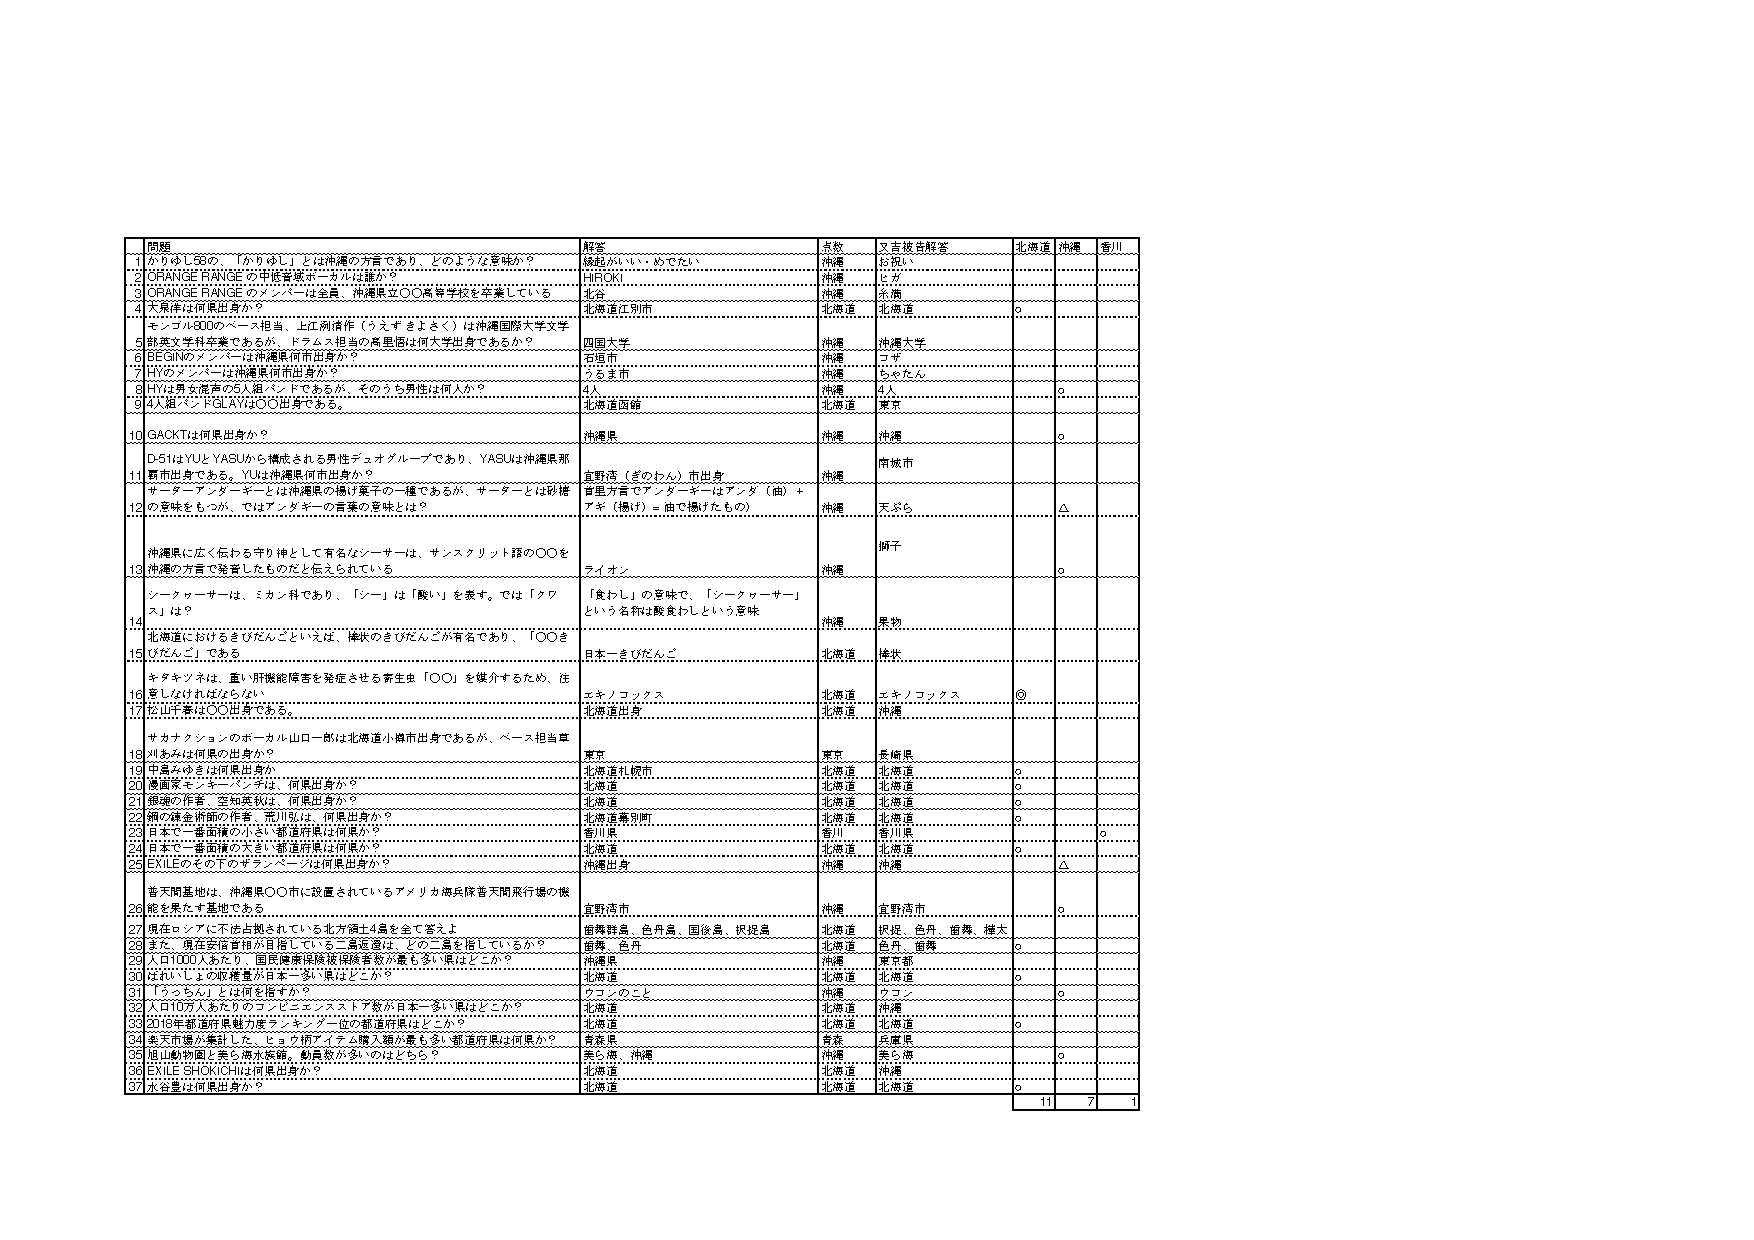
\includegraphics[clip,scale=0.9]{./section/Taira/figures/situgi}
  \caption{尋問一覧表。}
\label{situgi}
\end{figure}

(武田検事)つまり、求刑、一億十三億光年。\par
(裁判長)ん、これは有罪。\par
(又吉被告)そもそも、問題が悪い。沖縄は\CID{1624}\CID{1624}市と問うているのに北海道は北海道だけ。これは問題が悪い。\par
(武田検事)そんなことはない。\par

\subsection{結論}
最高裁へつづく
